\section{定制标注样式样板}
在前面几章中,我们每次标注尺寸时都需要按照\ref{sec:lianjieganshitu}节的尺寸样式设置步骤进行标注样式设置,其过程比较繁琐,能否有一种方法可以实现一次定制重复使用呢?要实现这样的要求,可利用AutoCAD的模板功能。下面是制作带有国家标准标注样式的AutoCAD模板的基本步骤。
\begin{procedure}
\item 新建文档

在AutoCAD中新建文档的方式有很多,常用的方式有:
\begin{itemize}
\item 键盘输入new\index{new,新建}
\item 
\includegraphics[scale=0.3]{keyctrl}+
\includegraphics[scale=0.3]{keyn}
\item 【文件】$\rightarrow $【新建】
\item 【标准】
\includegraphics[scale=0.45]{biaozhuntools}工具栏中的
\includegraphics[scale=0.45]{newtool}图标
\item 【快速访问】
\includegraphics[scale=0.45]{quicktools}中的
\includegraphics[scale=0.45]{newtool}图标
\end{itemize}

命令启动后弹出图\ref{fig:newfiletemplate}所示的选择样板对话框,选择acadiso.dwt文件并点击打开按钮。

\begin{figure}[htbp]
\centering
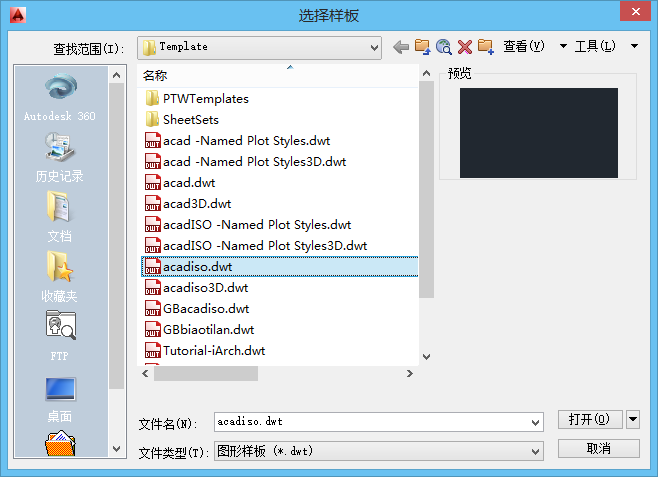
\includegraphics[scale=0.5]{newfiletemplate}
\caption{新建文件对话}\label{fig:newfiletemplate}
\end{figure}

\begin{lstlisting}
命令:new
\end{lstlisting}

\item 设置文字样式

按照\ref{sec:lianjieganshitu}节的方法设置文字样式。

\item 设置标注样式

按照\ref{sec:lianjieganshitu}节的方法设置标注样式。

\item 保存为样板文件

完成设置后,点击保存或另存为,弹出图\ref{fig:GBacadisotemplate}所示的图形另存为对话框,在文件下拉列表框中选择“AutoCAD 图形样板文件.dwt”,并以“GBacadiso.dwt”文件名进行保存,弹出图\ref{fig:GBtamplate}所示的样板选项对话框,在其中输入说明后点击确定即可生成样板文件。


\begin{figure}[htbp]
\centering
\begin{floatrow}[2]
\ffigbox{\caption{保存为样板}\label{fig:GBacadisotemplate}}{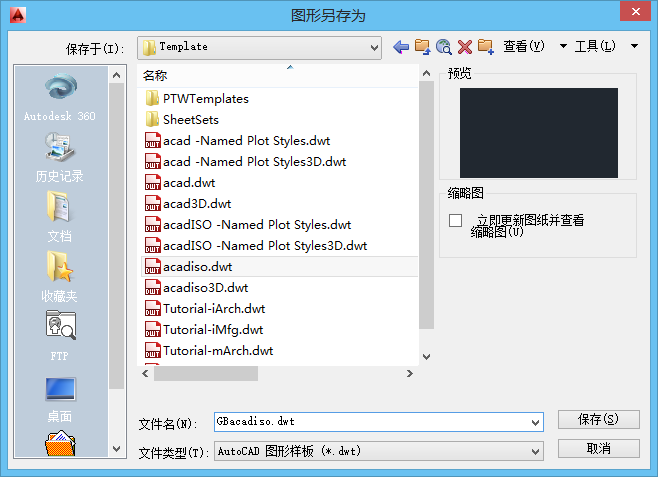
\includegraphics[scale=0.3]{GBacadisotemplate}}
\ffigbox{\caption{样板选项对话框}\label{fig:GBtamplate}}{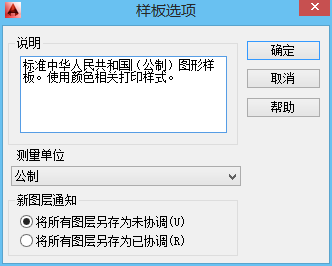
\includegraphics[scale=0.4]{GBtamplate}}
\end{floatrow}
\end{figure}

\item 关闭样板文件

完成样板文件定制后需要关闭。在新建文件时选择此样板文件来创建新文件,新文件就已经具备标准的文字样式设置和标注样式设置。
\end{procedure}
\endinput